\subsubsection{Preprocessing}
	The provided Kaggle data comes with a guarantee that the tweets are either about weather or are labelled in a way that indicates that they aren't about weather. So, there was no need to filter out entired tweets. But, as expected, a lot of the content of tweets aren't particularly important to our analysis. Stopwords like ``a'' and ``the'' are not worth considering in our algorithms. Using a predefined list of stopwords (reference mentioned in Appendix), we filtered out all stopwords from tweets. Moreover, we filtered out some common Twitter-specific jargon that bears no meaning in our problem, e.g. ``RT'' and ``@mention''.
	
	 Although capitalization may be indicative of strong emotions (and therefore helpful to sentiment), we've chosen to focus on the words themselves, so all words in each tweet are converted to lowercase. Lastly, all  punctuation symbols within a tweet are removed. Well, not quite \emph{all} punctuation...emoticons are comprised of punctuation marks and can be quite useful with regards to understanding sentiment, so all emoticons are kept in the tweets and treated as any other word.



\subsubsection{Important Words}
	The discriminative algorithms we use (SVM and decision trees) rely on translating our tweets into feature vectors, where each feature is a word of the vocabulary. Our vocabulary $V$ was very large (on the order of $10^7$), so it would be unwieldy to represent each tweet with a vector of length $|V|$, especially since some words aren't as important as others in determining weather/sentiment from tweets. To deal with this issue, we used class conditional probabilities from Naive Bayes (algorithm discussed later) to determine which words are most important in determining sentiment, when, and kind -- the notion of ``most important'' has to do with which words have a high probability of occuring given that, for example, the kind of weather is ``rainy''.

	The most important words for sentiment, when, and kind generated from this analysis are depicted in the below word clouds (larger words are more important than smaller ones). As we can see, most of these important words are indeed related to weather. For instance, it is unsurprising that the word ``good'' has high importance for sentiment, and ``storm'' has high importance for kind.

\begin{figure}[!htb]
\minipage{0.5\textwidth}
  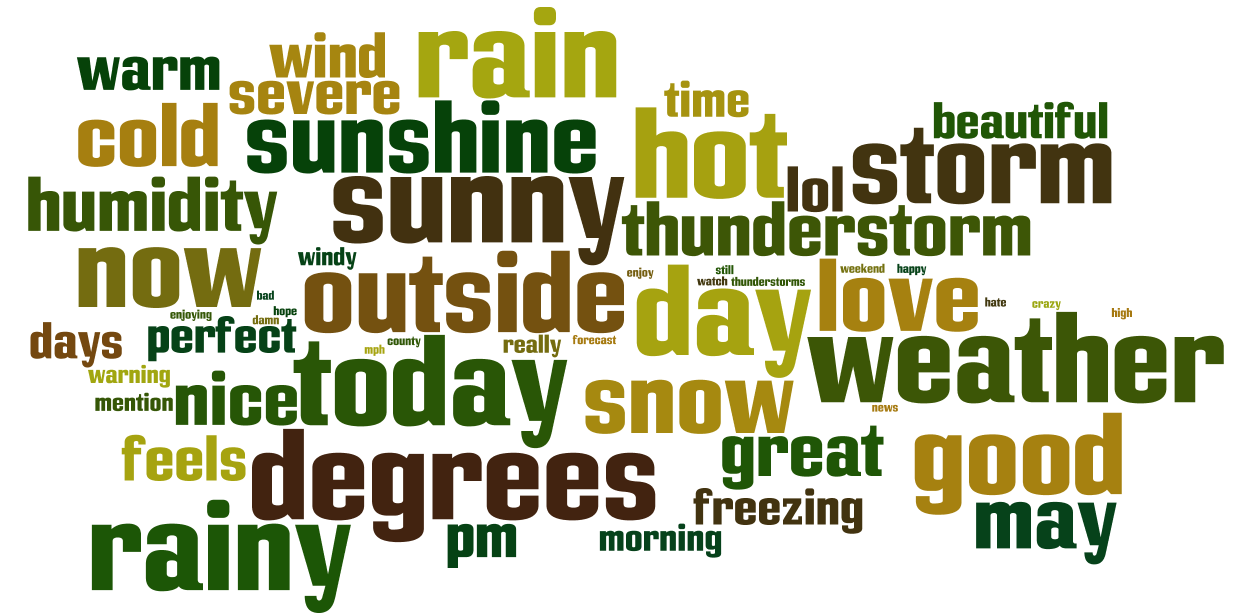
\includegraphics[width=\linewidth]{wordclouds/31sentiment}
  \caption{Top 30 ``sentiment'' words}\label{fig:awesome_image1}
\endminipage\hfill
\minipage{0.5\textwidth}
  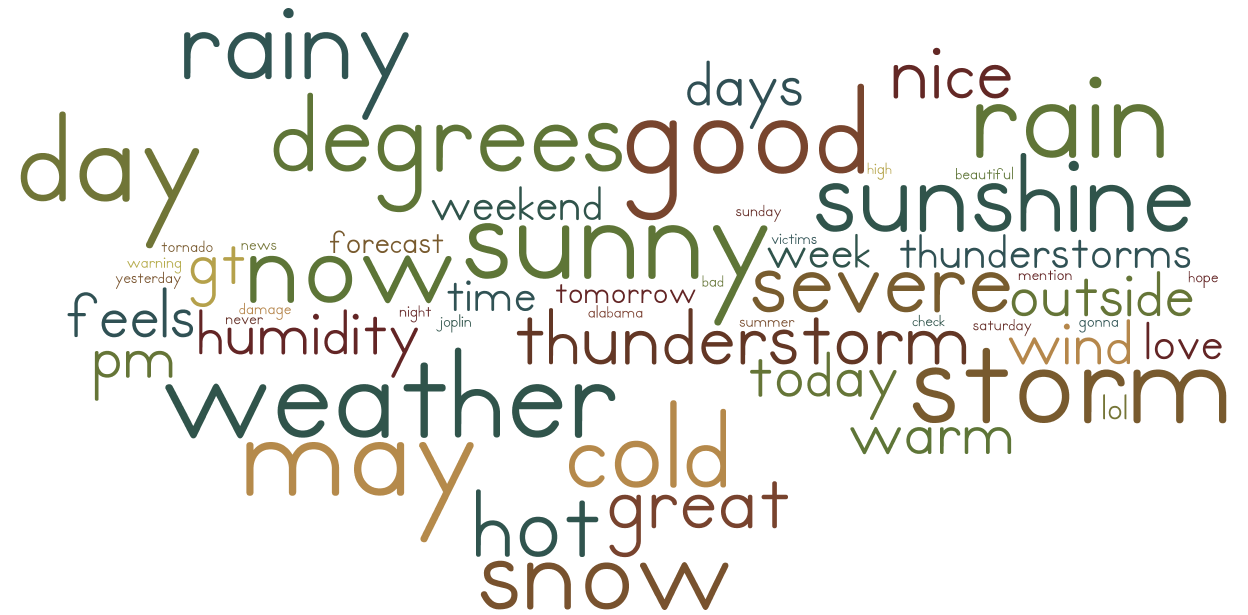
\includegraphics[width=\linewidth]{wordclouds/31when}
  \caption{Top 30 ``when'' words}\label{fig:awesome_image2}
\endminipage\hfill
\noindent\makebox[\textwidth][c]{%
\minipage{0.5\textwidth}%
  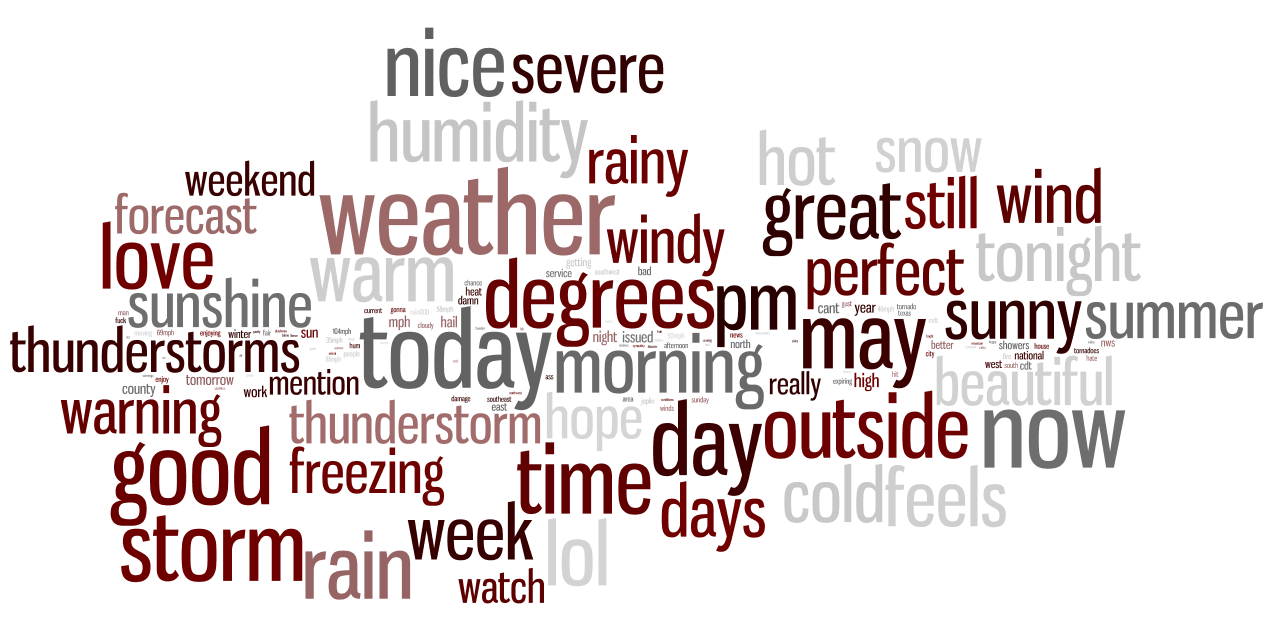
\includegraphics[width=\linewidth]{wordclouds/50kindwords}
  \caption{Top 50 ``kind'' words}\label{fig:awesome_image3}
\endminipage}
\end{figure}


\subsubsection{Data for MRF}
	We explore a method for tackling this problem using Markov Random Fields (MRF), which relies on location data and time data. The available Kaggle data doesn't have timestamps, so we utilized a separate dataset (referenced in Appendix). This data set is unlabelled and not weather-specific. To distill out the tweets related to weather, we removed all tweets that do not contain any words from the list of most important words for determining the kind of weather (gathering of important words discussed in previous subsection). The tweets were then labelled using decision trees (algorithm methodology discussed later), which did the best job of determining the kind of weather. Finally, we sent the remaining tweets through the same preprocessing specified in the ``Preprocessing'' subsection above.